\chapter{Шардинг}
\begin{epigraphs}
\qitem{Если ешь слона, не пытайся запихать его в рот целиком.}{Народная мудрость}
\end{epigraphs}
\section{Введение}
Шардинг~--- разделение данных на уровне ресурсов. Концепция шардинга заключается в логическом разделении данных по различным 
ресурсам исходя из требований к нагрузке.

Рассмотрим пример. Пусть у нас есть приложение с регистрацией пользователей, которое позволяет писать друг другу 
личные сообщения. Допустим оно очень популярно и много людей им пользуются ежедневно. Естественно, что таблица с личными 
сообщениями будет намного больше всех остальных таблиц в базе (скажем, будет занимать 90\% всех ресурсов). Зная это, 
мы можем подготовить для этой (только одной!) таблицы выделенный сервер помощнее, а остальные оставить на другом (послабее). 
Теперь мы можем идеально подстроить сервер для работы с одной специфической таблицей, постараться уместить ее в память, возможно, 
дополнительно партиционировать ее и т.д. Такое распределение называется вертикальным шардингом.

Что делать, если наша таблица с сообщениями стала настолько большой, что даже выделенный сервер под нее одну уже не спасает. 
Необходимо делать горизонтальный шардинг~--- т.е. разделение одной таблицы по разным ресурсам. Как это выглядит на практике? 
Все просто. На разных серверах у нас будет таблица с одинаковой структурой, но разными данными. Для нашего случая с сообщениями, 
мы можем хранить первые 10 миллионов сообщений на одном сервере, вторые 10 - на втором и т.д. Т.е. необходимо иметь критерий 
шардинга~--- какой-то параметр, который позволит определять, на каком именно сервере лежат те или иные данные.

Обычно, в качестве параметра шардинга выбирают ID пользователя (user\_id)~--- это позволяет делить данные по серверам равномерно 
и просто. Т.о. при получении личных сообщений пользователей алгоритм работы будет такой:
\begin{itemize}
\item Определить, на каком сервере БД лежат сообщения пользователя исходя из user\_id
\item Инициализировать соединение с этим сервером
\item Выбрать сообщения
\end{itemize}

Задачу определения конкретного сервера можно решать двумя путями:
\begin{itemize}
\item Хранить в одном месте хеш-таблицу с соответствиями <<пользователь=сервер>>. Тогда, при определении сервера, нужно будет 
выбрать сервер из этой таблицы. В этом случае узкое место~--- это большая таблица соответствия, которую нужно хранить в одном месте. 
Для таких целей очень хорошо подходят базы данных <<ключ=значение>>
\item Определять имя сервера с помощью числового (буквенного) преобразования. Например, можно вычислять номер сервера, 
как остаток от деления на определенное число (количество серверов, между которыми Вы делите таблицу). В этом случае узкое место~--- 
это проблема добавления новых серверов~--- Вам придется делать перераспределение данных между новым количеством серверов.
\end{itemize}

Для шардинга не существует решения на уровне известных платформ, т.к. это весьма специфическая для отдельно взятого приложения задача.

Естественно, делая горизонтальный шардинг, Вы ограничиваете себя в возможности выборок, которые требуют 
пересмотра всей таблицы (например, последние посты в блогах людей будет достать невозможно, если таблица постов шардится). 
Такие задачи придется решать другими подходами. Например, для описанного примера, можно при появлении нового поста, заносить 
его ID в общий стек, размером в 100 элементом.

Горизонтальный шардинг имеет одно явное преимущество~--- он бесконечно масштабируем.
Для создания шардинга PostgreSQL существует несколько решений:
\begin{itemize}
\item \href{http://postgres-xc.sourceforge.net/}{Postgres-XC}
\item \href{http://plproxy.projects.postgresql.org/doc/tutorial.html}{PL/Proxy}
\item \href{http://db.cs.yale.edu/hadoopdb/hadoopdb.html}{HadoopDB (Shared-nothing clustering)}
\item \href{http://www.greenplum.com/products/greenplum-database}{Greenplum Database}
\end{itemize}


\section{PL/Proxy}
\label{sec:plproxy}
PL/Proxy представляет собой прокси-язык для удаленного вызова процедур и партицирования данных между разными базами.
Основная идея его использования заключается в том, что появляется возможность вызывать функции, расположенные в удаленных
базах, а также свободно работать с кластером баз данных (например, вызвать функцию на всех узлах кластера, или на
случайном узле, или на каком-то одном определенном).

Чем PL/Proxy может быть полезен? Он существенно упрощает горизонтальное масштабирование системы.
Становится удобным разделять таблицу с пользователями, например, по первой латинской букве имени~--- на 26 узлов.
При этом приложение, которое работает непосредственно с прокси-базой, ничего не будет замечать: запрос на авторизацию,
например, сам будет направлен прокси-сервером на нужный узел. То есть администратор баз данных может проводить масштабирование
системы практически независимо от разработчиков приложения.

PL/Proxy позволяет полностью решить проблемы масштабирования OLTP систем. В систему легко вводится резервирование с
failover-ом не только по узлам, но и по самим прокси-серверам, каждый из которых работает со всеми узлами.

Недостатки и ограничения:
\begin{itemize}
\item все запросы и вызовы функций вызываются в autocommit-режиме на удаленных серверах
\item в теле функции разрешен только один SELECT; при необходимости нужно писать отдельную процедуру
\item при каждом вызове прокси-сервер стартует новое соединение к бакенд-серверу; в высоконагруженных системах
целесообразно использовать менеджер для кеширования соединений к бакенд-серверам, для этой цели идеально подходит PgBouncer
\item изменение конфигурации кластера (количества партиций, например) требует перезапуска прокси-сервера
\end{itemize}


\subsection{Установка}
\begin{enumerate}
\item Скачать PL/Proxy\footnote{http://pgfoundry.org/projects/plproxy} и распаковать.
\item Собрать PL/Proxy командами make и make install.
\end{enumerate}

Так же можно установить PL/Proxy из репозитория пакетов.
Например в Ubuntu Server достаточно выполнить команду для PostgreSQL 8.4:
\begin{lstlisting}[label=lst:plproxy1,caption=Установка]
sudo aptitude install postgresql-8.4-plproxy
\end{lstlisting}

\subsection{Настройка}
Для примера настройки используется 3 сервера PostgreSQL. 2 сервера пусть будут node1 и node2,
а главный, что будет проксировать запросы на два других~--- proxy.
Для корректной работы pl/proxy рекомендуется использовать количество нод равное степеням двойки.
База данных будет называтся plproxytest, а таблица в ней~--- users. Начнем!

Для начала настроим node1 и node2. Команды написанные ниже нужно выполнять на каждой ноде.

Создадим базу данных plproxytest(если её ещё нет):
\begin{lstlisting}[language=SQL,label=lst:plproxy2,caption=Настройка]
CREATE DATABASE plproxytest
     WITH OWNER = postgres
       ENCODING = 'UTF8';
\end{lstlisting}

Добавляем табличку users:
\begin{lstlisting}[language=SQL,label=lst:plproxy3,caption=Настройка]
CREATE TABLE public.users
  (
   username character varying(255),
   email character varying(255)
  )
  WITH (OIDS=FALSE);
ALTER TABLE public.users OWNER TO postgres;
\end{lstlisting}

Теперь создадим функцию для добавления данных в таблицу users:
\begin{lstlisting}[language=SQL,label=lst:plproxy4,caption=Настройка]
CREATE OR REPLACE FUNCTION public.insert_user(i_username text,
i_emailaddress   text)
RETURNS integer AS
$BODY$
INSERT INTO public.users (username, email) VALUES ($1,$2);
    SELECT 1;
$BODY$
  LANGUAGE 'sql' VOLATILE;
ALTER FUNCTION public.insert_user(text, text) OWNER TO postgres;
\end{lstlisting}

С настройкой нодов закончено. Приступим к серверу proxy.

Как и на всех нодах, на главном сервере (proxy) должна присутствовать база данных:
\begin{lstlisting}[language=SQL,label=lst:plproxy5,caption=Настройка]
CREATE DATABASE plproxytest
     WITH OWNER = postgres
       ENCODING = 'UTF8';
\end{lstlisting}

Теперь надо указать серверу что эта база данных управляется с помощью pl/proxy:
\begin{lstlisting}[language=SQL,label=lst:plproxy6,caption=Настройка]
CREATE OR REPLACE FUNCTION public.plproxy_call_handler()
  RETURNS language_handler AS
'$libdir/plproxy', 'plproxy_call_handler'
  LANGUAGE 'c' VOLATILE
COST 1;
ALTER FUNCTION public.plproxy_call_handler()
OWNER TO postgres;
-- language
CREATE LANGUAGE plproxy HANDLER plproxy_call_handler;
CREATE LANGUAGE plpgsql;
\end{lstlisting}

Также, для того что бы сервер знал где и какие ноды у него есть, надо создать 3 сервисные функции, которые pl/proxy будет использовать в своей работе. Первая функция~--- конфиг для кластера баз данных. Тут указываются параметры через key-value:
\begin{lstlisting}[language=SQL,label=lst:plproxy7,caption=Настройка]
CREATE OR REPLACE FUNCTION public.get_cluster_config
(IN cluster_name text,   OUT "key" text, OUT val text)
  RETURNS SETOF record AS
$BODY$
BEGIN
  -- lets use same config for all clusters
  key := 'connection_lifetime';
  val := 30*60; -- 30m
  RETURN NEXT;
  RETURN;
END;
$BODY$
  LANGUAGE 'plpgsql' VOLATILE
  COST 100
  ROWS 1000;
ALTER FUNCTION public.get_cluster_config(text)
OWNER TO postgres;
\end{lstlisting}

Вторая важная функция, код которой надо будет подправить. В ней надо будет указать DSN нод:
\begin{lstlisting}[language=SQL,label=lst:plproxy8,caption=Настройка]
CREATE OR REPLACE FUNCTION
public.get_cluster_partitions(cluster_name text)
  RETURNS SETOF text AS
$BODY$
BEGIN
  IF cluster_name = 'usercluster' THEN
    RETURN NEXT 'dbname=plproxytest host=node1 user=postgres';
    RETURN NEXT 'dbname=plproxytest host=node2 user=postgres';
    RETURN;
  END IF;
  RAISE EXCEPTION 'Unknown cluster';
END;
$BODY$
  LANGUAGE 'plpgsql' VOLATILE
  COST 100
  ROWS 1000;
ALTER FUNCTION public.get_cluster_partitions(text)
OWNER TO postgres;
\end{lstlisting}

И последняя:
\begin{lstlisting}[language=SQL,label=lst:plproxy9,caption=Настройка]
CREATE OR REPLACE FUNCTION
public.get_cluster_version(cluster_name text)
  RETURNS integer AS
$BODY$
BEGIN
  IF cluster_name = 'usercluster' THEN
    RETURN 1;
  END IF;
  RAISE EXCEPTION 'Unknown cluster';
END;
$BODY$
  LANGUAGE 'plpgsql' VOLATILE
  COST 100;
ALTER FUNCTION public.get_cluster_version(text)
OWNER TO postgres;
\end{lstlisting}

Ну и собственно самая главная функция, которая будет вызываться уже непосредственно в приложении:
\begin{lstlisting}[language=SQL,label=lst:plproxy10,caption=Настройка]
CREATE OR REPLACE FUNCTION
public.insert_user(i_username text, i_emailaddress text)
  RETURNS integer AS
$BODY$
  CLUSTER 'usercluster';
  RUN ON hashtext(i_username);
$BODY$
  LANGUAGE 'plproxy' VOLATILE
  COST 100;
ALTER FUNCTION public.insert_user(text, text)
OWNER TO postgres;
\end{lstlisting}

Все готово. Подключаемся к серверу proxy и заносим данные в базу:
\begin{lstlisting}[language=SQL,label=lst:plproxy11,caption=Настройка]
SELECT insert_user('Sven','sven@somewhere.com');
SELECT insert_user('Marko', 'marko@somewhere.com');
SELECT insert_user('Steve','steve@somewhere.com');
\end{lstlisting}

Пробуем извлечь данные.
Для этого напишем новую серверную функцию:
\begin{lstlisting}[language=SQL,label=lst:plproxy12,caption=Настройка]
CREATE OR REPLACE FUNCTION
public.get_user_email(i_username text)
 RETURNS SETOF text AS
$BODY$
 CLUSTER 'usercluster';
 RUN ON hashtext(i_username) ;
 SELECT email FROM public.users
 WHERE username = i_username;
$BODY$
 LANGUAGE 'plproxy' VOLATILE
 COST 100
 ROWS 1000;
ALTER FUNCTION public.get_user_email(text)
OWNER TO postgres;
\end{lstlisting}

И попробуем её вызвать:
\begin{lstlisting}[language=SQL,label=lst:plproxy13,caption=Настройка]
select plproxy.get_user_email('Steve');
\end{lstlisting}

Если потом подключиться к каждой ноде отдельно, то можно четко увидеть, что данные users разбросаны по таблицам каждой ноды.

\subsection{Все ли так просто?}
Как видно на тестовом примере ничего сложного в работе с pl/proxy нет.
Но, я думаю все кто смог дочитать до этой строчки уже поняли что в реальной жизни все не так просто.
Представьте что у вас 16 нод. Это же надо как-то синхронизировать код функций. А что если ошибка закрадётся~---
как её оперативно исправлять?

Этот вопрос был задан и на конференции Highload++ 2008, на что Аско Ойя ответил что соответствующие средства
уже реализованы внутри самого Skype, но ещё не достаточно готовы для того что бы отдавать их на суд сообществу opensource.

Второй проблема, которая не дай бог коснётся вас при разработке такого рода системы, это проблема перераспределения данных
в тот момент когда нам захочется добавить ещё нод в кластер.
Планировать эту масштабную операцию придётся очень тщательно, подготовив все сервера заранее,
занеся данные и потом в один момент подменив код функции get\_cluster\_partitions.
\section{Postgres-XC}
\label{sec:postgres-xc}

Postgres-XC~-- система для создания мульти-мастер кластеров, работающих в синхронном режиме~-- все узлы всегда содержат актуальные данные. Postgres-XC поддерживает опции для увеличения масштабирования кластера как при преобладании операций записи, так и при основной нагрузке на чтение данных: поддерживается выполнение транзакций с распараллеливанием на несколько узлов, за целостностью транзакций в пределах всего кластера отвечает специальный узел GTM (Global Transaction Manager).

Измерение производительности показало, что КПД кластера Postgres-XC составляет примерно 64\%, т.е. кластер из 10 серверов позволяет добиться увеличения производительности системы в целом в 6.4 раза, относительно производительности одного сервера (цифры приблизительные).

Система не использует в своей работе триггеры и представляет собой набор дополнений и патчей к PostgreSQL, дающих возможность в прозрачном режиме обеспечить работу в кластере стандартных приложений, без их дополнительной модификации и адаптации (полная совместимость с PostgreSQL API). Кластер состоит из одного управляющего узла (GTM), предоставляющего информацию о состоянии транзакций, и произвольного набора рабочих узлов, каждый из которых в свою очередь состоит из координатора и обработчика данных (обычно эти элементы реализуются на одном сервере, но могут быть и разделены).

Хоть Postgres-XC и выглядит похожим на MultiMaster, но он им не является. Все сервера кластера должны быть соединены сетью с минимальными задержками, никакое географически-распределенное решение с разумной производительностью построить на нем невозможно (это важный момент).

\subsection{Архитектура}

\begin{figure}[ht!]
  \center{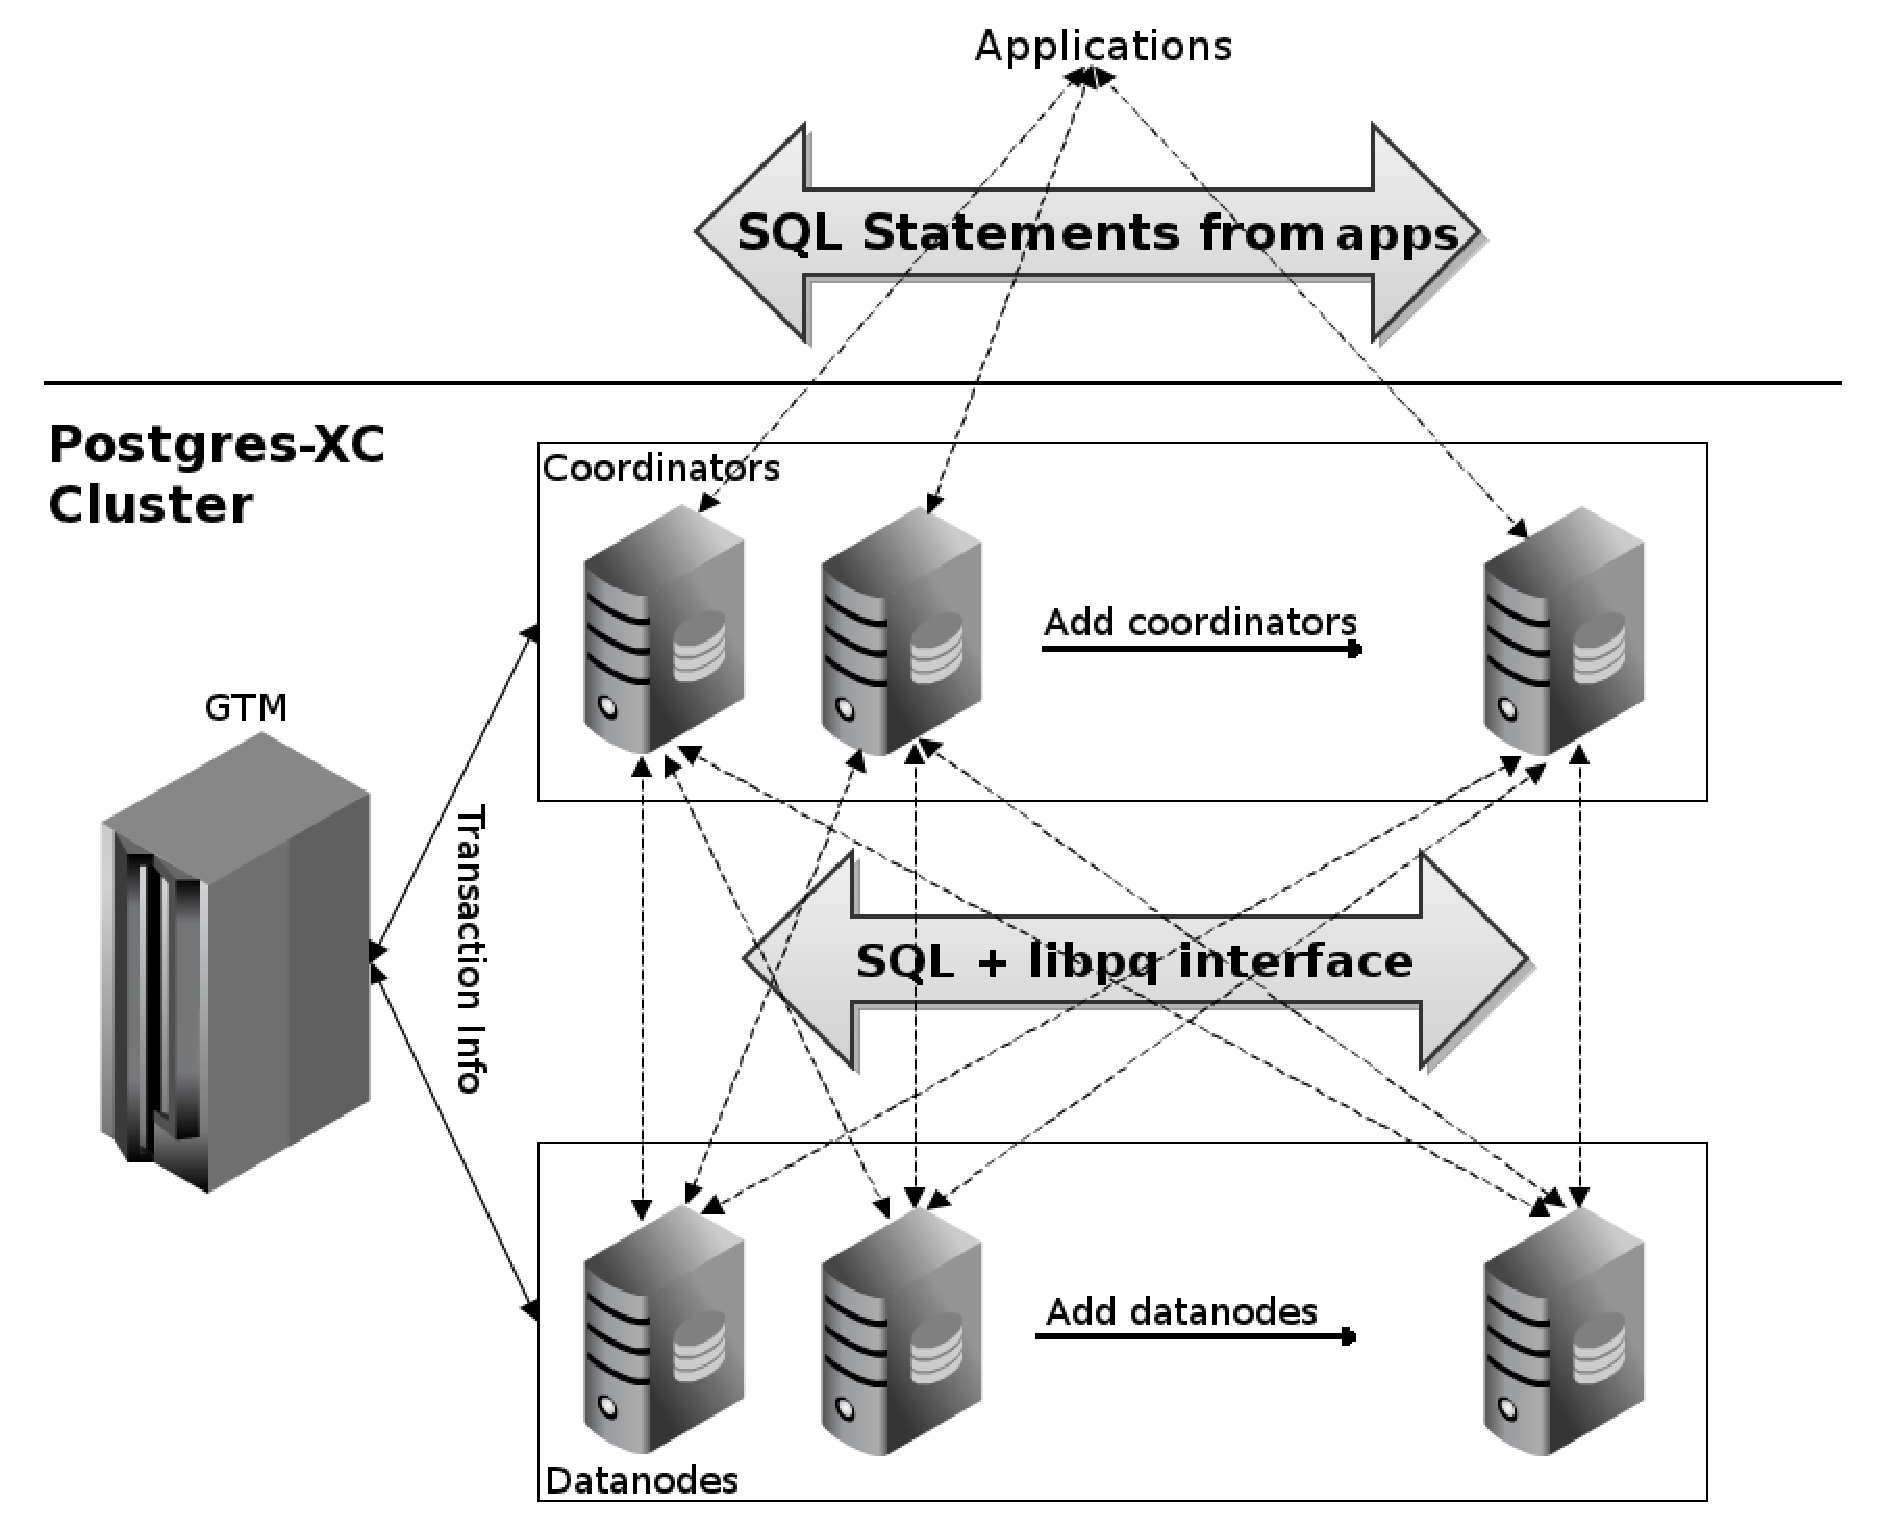
\includegraphics[width=1\textwidth]{postgres-xc-arch.pdf}}
  \caption{Архитектура Postgres-XC}
  \label{fig:postgres-xc1}
\end{figure}

Рис.~\ref{fig:postgres-xc1} показывает архитектуру Postgres-XC с тремя её основными компонентами:

\begin{enumerate}
  \item Глобальный менеджер транзакций (GTM)~--- собирает и обрабатывает информацию о транзакциях в Postgres-XC, решает вопросы глобального идентификатора транзакции по операциям (для поддержания согласованного представления базы данных на всех узлах). Он обеспечивает поддержку других глобальных данных, таких как последовательности и временные метки. Он хранит данные пользователя, за исключением управляющей информации.
  \item Координаторы (coordinators)~--- обеспечивают точку подключения для клиента (приложения). Они несут ответственность за разбор и выполнение запросов от клиентов и возвращение результатов (при необходимости). Они не хранят пользовательские данные, а собирают их из обработчиков данных (datanodes) с помощью запросов SQL через PostgreSQL интерфейс. Координаторы также обрабатывают данные, если требуется, и даже управляют двухфазной фиксацией. Координаторы используются также для разбора запросов, составления планов запросов, поиска данных и т.д.
  \item Обработчики данных (datanodes)~--- обеспечивают сохранение пользовательских данных. Datanodes выполняют запросы от координаторов и возвращают им полученный результат.
\end{enumerate}

\subsection{Установка}

Установить Postgres-XC можно из \href{http://postgres-x2.github.io/}{исходников} или же из пакетов системы. Например в Ubuntu 14.04 можно установить postgres-xc так:

\begin{lstlisting}[language=Bash,label=lst:postgres-xc1,caption=Установка Postgres-XC]
$ sudo apt-get install postgres-xc postgres-xc-client postgres-xc-contrib postgres-xc-server-dev
\end{lstlisting}

По умолчанию он создаст один координатор и два обработчика данных.

\subsection{Распределение данных и масштабируемость}

Postgres-XC предусматривает два способа хранения данных в таблицах:

\begin{figure}[ht!]
  \center{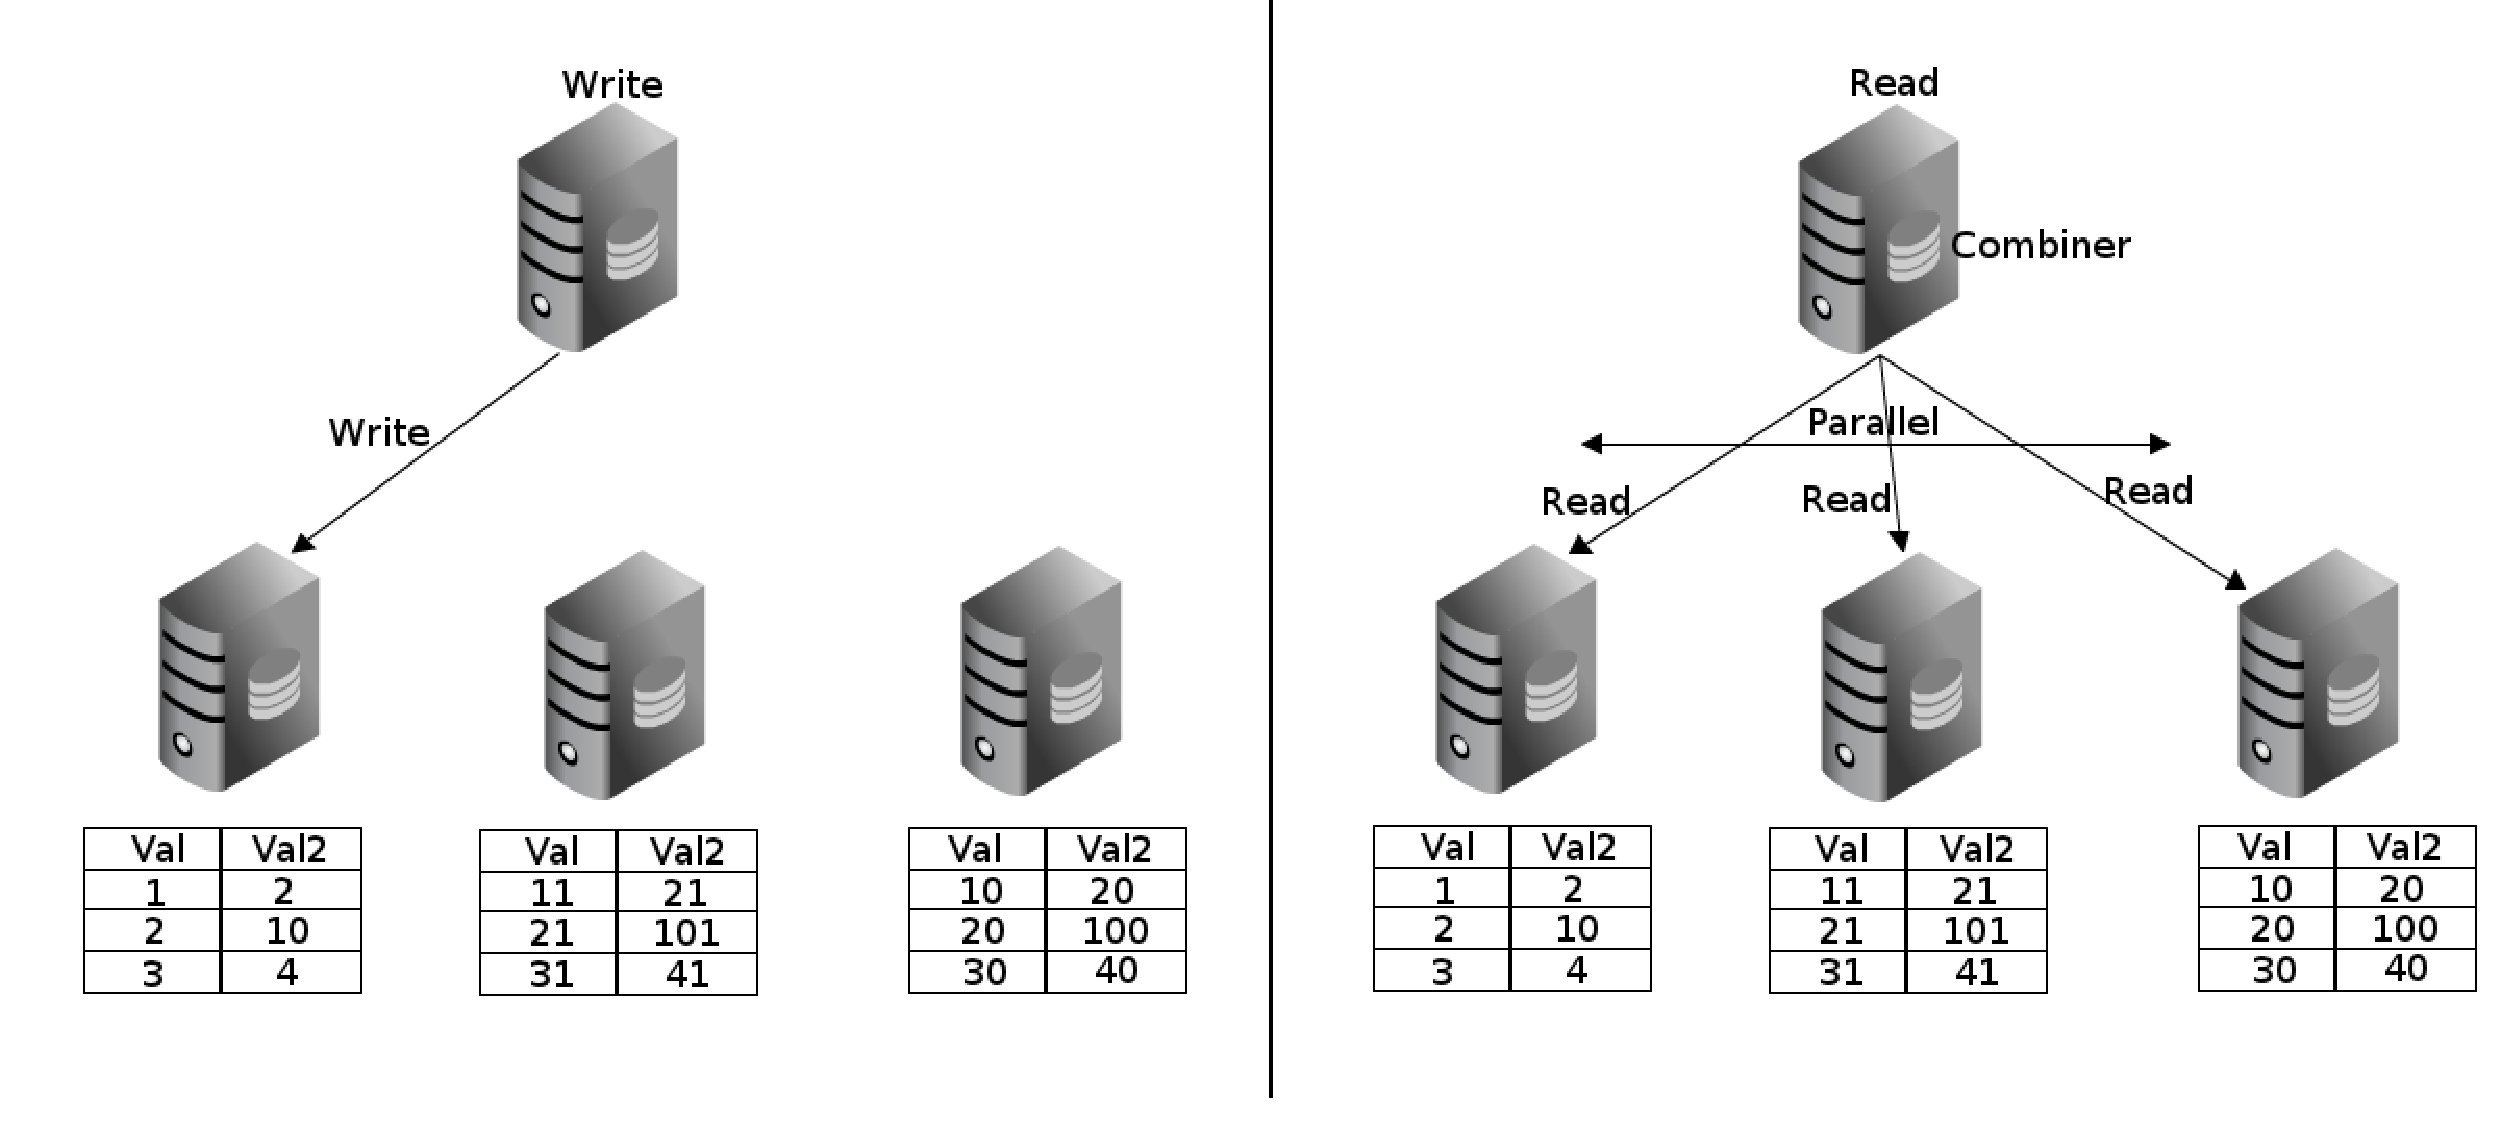
\includegraphics[width=1\textwidth]{postgres-xc-02.pdf}}
  \caption{Распределенные таблицы}
  \label{fig:postgres-xc2}
\end{figure}

\begin{figure}[ht!]
  \center{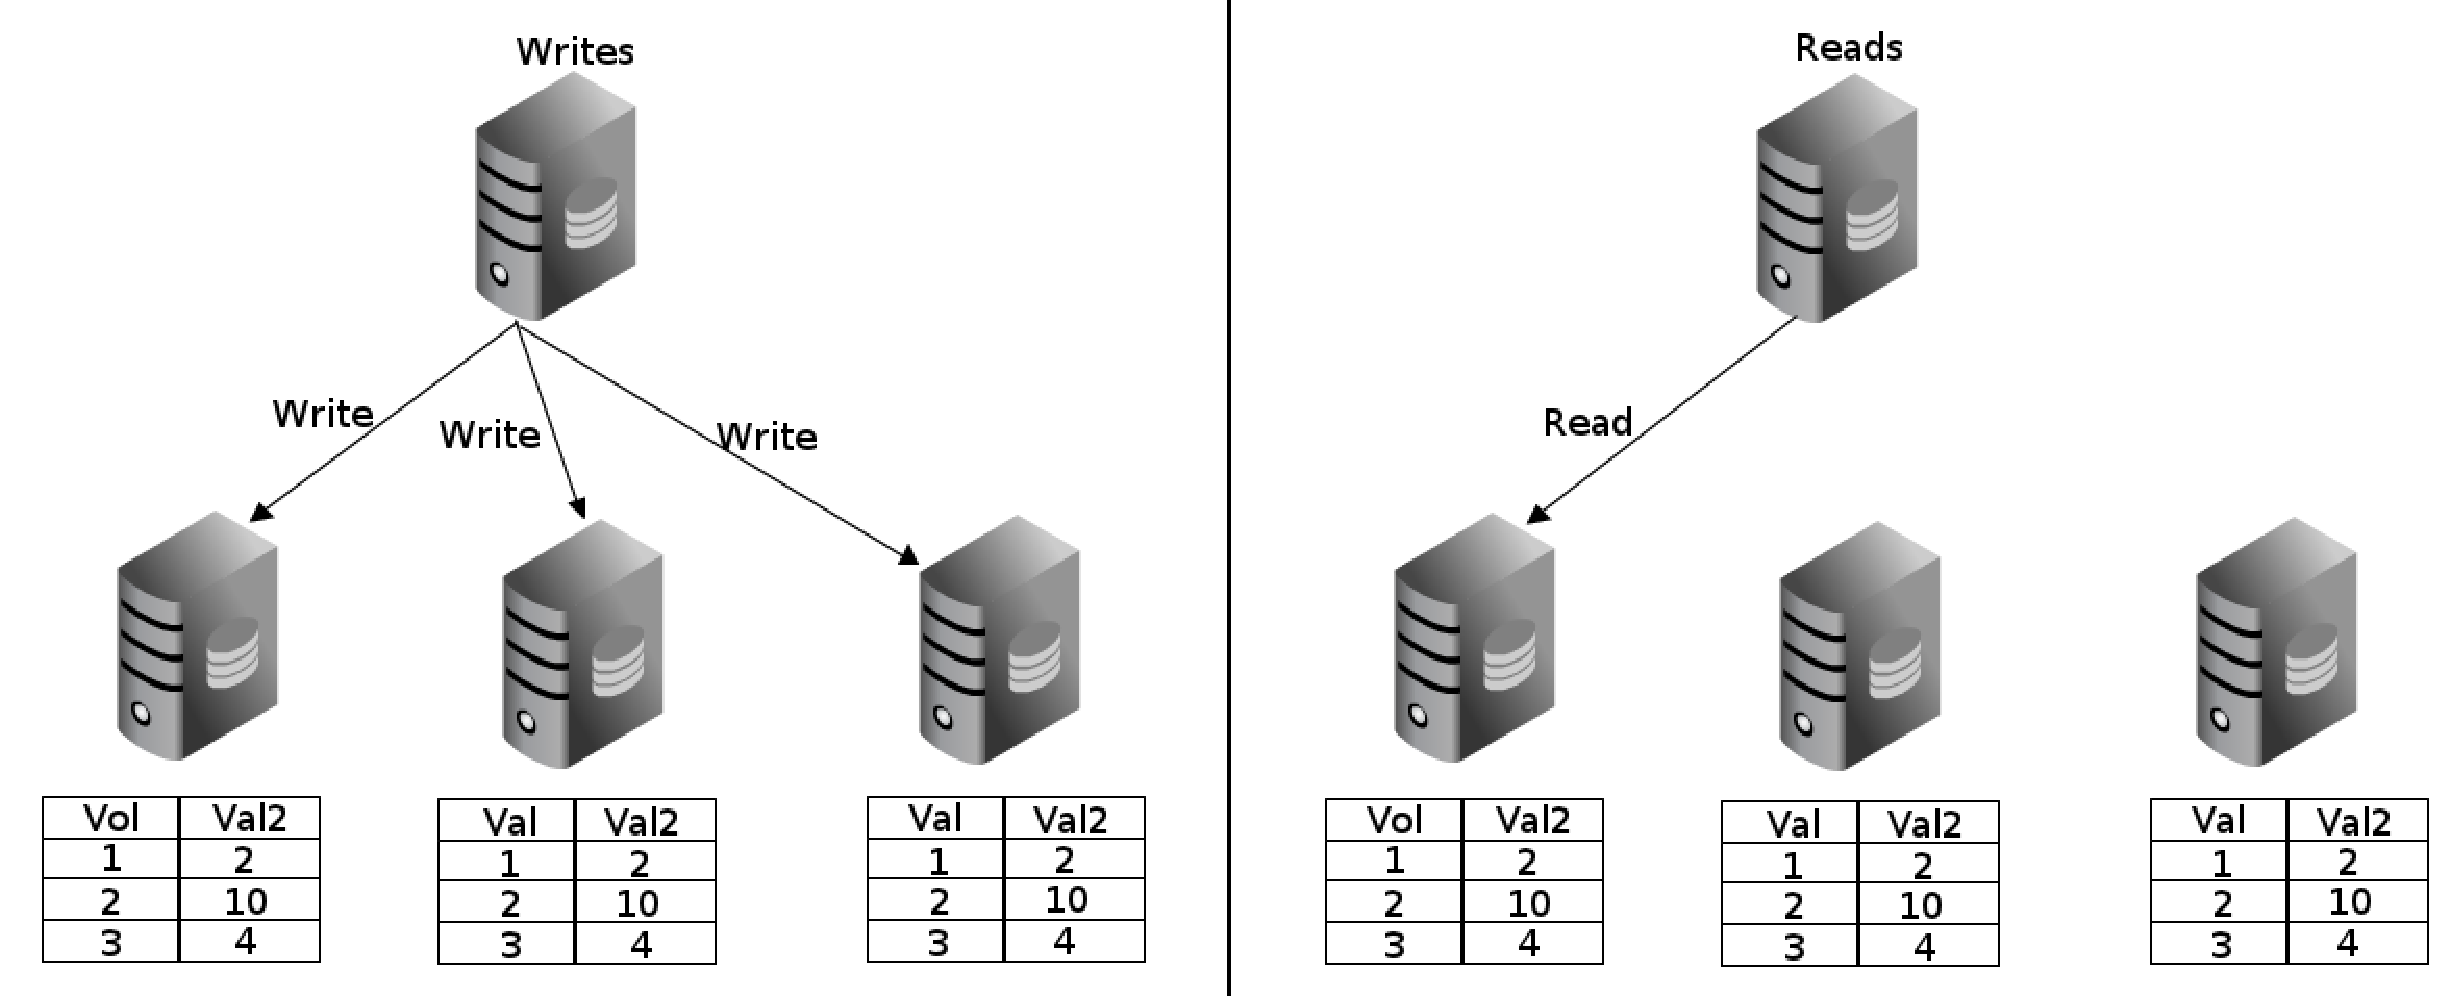
\includegraphics[width=1\textwidth]{postgres-xc-03.pdf}}
  \caption{Реплицированные таблицы}
  \label{fig:postgres-xc3}
\end{figure}

\begin{enumerate}
  \item Распределенные таблицы (distributed tables, рис.~\ref{fig:postgres-xc2}): данные по таблице распределяются на указанный набор обработчиков данных с использованием указанной стратегии (hash, round-robin, modulo). Каждая запись в таблице находится только на одном обработчике данных. Параллельно могут быть записаны или прочитаны данные с различных обработчиков данных. За счет этого значительно улучшена производительность на запись и чтение;
  \item Реплицированные таблицы (replicated tables, рис.~\ref{fig:postgres-xc3}): данные по таблице реплицируется (клонируются) на указанный набор обработчиков данных. Каждая запись в таблице находится на всех обработчиках данных (которые были указаны) и любые изменения дублируются на все обработчики данных. Так как все данные доступны на любом обработчике данных, координатор может собрать все данные из одного узла, что позволяет направить различные запросы на различные обработчики данных. Таким образом создается балансировка нагрузки и увеличения пропускной способности на чтение.
\end{enumerate}

\subsection{Таблицы и запросы к ним}

После установки работа с Postgres-XC ведется как с обыкновенным PostgreSQL. Подключаться для работы с данными нужно только к координаторам (по умолчанию координатор работает на порту 5432). Для начала создадим распределенные таблицы.

\begin{lstlisting}[language=SQL,label=lst:postgres-xc2,caption=Создание распределенных таблиц]
CREATE TABLE
users_with_hash (id SERIAL, type INT, ...)
DISTRIBUTE by HASH(id);

CREATE TABLE
users_with_modulo (id SERIAL, type INT, ...)
DISTRIBUTE by MODULO(id);

CREATE TABLE
users_with_rrobin (id SERIAL, type INT, ...)
DISTRIBUTE by ROUNDROBIN;
\end{lstlisting}

На листинге~\ref{lst:postgres-xc2} создано 3 распределенные таблицы:

\begin{enumerate}
  \item Таблица \lstinline!users_with_hash! распределяется по хешу значения из указанного поля в таблице (тут указано поле id) по обработчикам данных. Вот как распределились первые 15 значений:

\begin{lstlisting}[language=SQL,label=lst:postgres-xc3,caption=Данные с координатора и обработчиков данных]
# координатор
$ psql
# SELECT id, type from users_with_hash ORDER BY id;
 id   | type
-------+-------
     1 |   946
     2 |   153
     3 |   484
     4 |   422
     5 |   785
     6 |   906
     7 |   973
     8 |   699
     9 |   434
    10 |   986
    11 |   135
    12 |  1012
    13 |   395
    14 |   667
    15 |   324

# первый обработчик данных
$ psql -p15432
# SELECT id, type from users_with_hash ORDER BY id;
  id  | type
------+-------
    1 |   946
    2 |   153
    5 |   785
    6 |   906
    8 |   699
    9 |   434
   12 |  1012
   13 |   395
   15 |   324

# второй обработчик данных
$ psql -p15433
# SELECT id, type from users_with_hash ORDER BY id;
 id   | type
-------+-------
     3 |   484
     4 |   422
     7 |   973
    10 |   986
    11 |   135
    14 |   667
\end{lstlisting}

  \item Таблица \lstinline!users_with_modulo! распределяется по модулю значения из указанного поля в таблице (тут указано поле id) по обработчикам данных. Вот как распределились первые 15 значений:

\begin{lstlisting}[language=SQL,label=lst:postgres-xc4,caption=Данные с координатора и обработчиков данных]
# координатор
$ psql
# SELECT id, type from users_with_modulo ORDER BY id;
 id   | type
-------+-------
     1 |   883
     2 |   719
     3 |    29
     4 |   638
     5 |   363
     6 |   946
     7 |   440
     8 |   331
     9 |   884
    10 |   199
    11 |    78
    12 |   791
    13 |   345
    14 |   476
    15 |   860

# первый обработчик данных
$ psql -p15432
# SELECT id, type from users_with_modulo ORDER BY id;
  id   | type
-------+-------
     2 |   719
     4 |   638
     6 |   946
     8 |   331
    10 |   199
    12 |   791
    14 |   476

# второй обработчик данных
$ psql -p15433
# SELECT id, type from users_with_modulo ORDER BY id;
  id  | type
------+-------
    1 |   883
    3 |    29
    5 |   363
    7 |   440
    9 |   884
   11 |    78
   13 |   345
   15 |   860
\end{lstlisting}

  \item Таблица \lstinline!users_with_rrobin! распределяется циклическим способом(round-robin) по обработчикам данных. Вот как распределились первые 15 значений:

\begin{lstlisting}[language=SQL,label=lst:postgres-xc5,caption=Данные с координатора и обработчиков данных]
# координатор
$ psql
# SELECT id, type from users_with_rrobin ORDER BY id;
 id   | type
-------+-------
     1 |   890
     2 |   198
     3 |   815
     4 |   446
     5 |    61
     6 |   337
     7 |   948
     8 |   446
     9 |   796
    10 |   422
    11 |   242
    12 |   795
    13 |   314
    14 |   240
    15 |   733

# первый обработчик данных
$ psql -p15432
# SELECT id, type from users_with_rrobin ORDER BY id;
  id   | type
-------+-------
     2 |   198
     4 |   446
     6 |   337
     8 |   446
    10 |   422
    12 |   795
    14 |   240

# второй обработчик данных
$ psql -p15433
# SELECT id, type from users_with_rrobin ORDER BY id;
  id  | type
------+-------
    1 |   890
    3 |   815
    5 |    61
    7 |   948
    9 |   796
   11 |   242
   13 |   314
   15 |   733
\end{lstlisting}

\end{enumerate}

Теперь создадим реплицированную таблицу:

\begin{lstlisting}[language=SQL,label=lst:postgres-xc20,caption=Создание реплицированной таблицы]
CREATE TABLE
users_replicated (id SERIAL, type INT, ...)
DISTRIBUTE by REPLICATION;
\end{lstlisting}

Естественно данные идентичны на всех обработчиках данных:

\begin{lstlisting}[language=SQL,label=lst:postgres-xc21,caption=Данные с координатора и обработчиков данных]
# SELECT id, type from users_replicated  ORDER BY id;
  id   | type
-------+-------
     1 |    75
     2 |   262
     3 |   458
     4 |   779
     5 |   357
     6 |    51
     7 |   249
     8 |   444
     9 |   890
    10 |   810
    11 |   809
    12 |   166
    13 |   605
    14 |   401
    15 |    58
\end{lstlisting}

Рассмотрим как выполняются запросы для таблиц. Выберем все записи из распределенной таблицы:

\begin{lstlisting}[language=SQL,label=lst:postgres-xc6,caption=Выборка записей из распределенной таблицы]
# EXPLAIN VERBOSE SELECT * from users_with_modulo ORDER BY id;
                                      QUERY PLAN
--------------------------------------------------------------------------------------
 Sort  (cost=49.83..52.33 rows=1000 width=8)
   Output: id, type
   Sort Key: users_with_modulo.id
   ->  Result  (cost=0.00..0.00 rows=1000 width=8)
         Output: id, type
         ->  Data Node Scan on users_with_modulo  (cost=0.00..0.00 rows=1000 width=8)
               Output: id, type
               Node/s: dn1, dn2
               Remote query: SELECT id, type FROM ONLY users_with_modulo WHERE true
(9 rows)
\end{lstlisting}

Как видно на листинге~\ref{lst:postgres-xc6} координатор собирает данные из обработчиков данных, а потом собирает их вместе.

Подсчет суммы с группировкой по полю из распределенной таблицы:

\begin{lstlisting}[language=SQL,label=lst:postgres-xc7,caption=Выборка записей из распределенной таблицы]
# EXPLAIN VERBOSE SELECT sum(id) from users_with_modulo GROUP BY type;
                                                                      QUERY PLAN
------------------------------------------------------------------------------------------------------------------------------------------------------
 HashAggregate  (cost=5.00..5.01 rows=1 width=8)
   Output: pg_catalog.sum((sum(users_with_modulo.id))), users_with_modulo.type
   ->  Materialize  (cost=0.00..0.00 rows=0 width=0)
         Output: (sum(users_with_modulo.id)), users_with_modulo.type
         ->  Data Node Scan on "__REMOTE_GROUP_QUERY__"  (cost=0.00..0.00 rows=1000 width=8)
               Output: sum(users_with_modulo.id), users_with_modulo.type
               Node/s: dn1, dn2
               Remote query: SELECT sum(group_1.id), group_1.type  FROM (SELECT id, type FROM ONLY users_with_modulo WHERE true) group_1 GROUP BY 2
(8 rows)
\end{lstlisting}

JOIN между и с участием реплицированных таблиц, а также JOIN между распределенными по одному и тому же полю в таблицах будет выполняются на обработчиках данных. Но JOIN с участием распределенных таблиц по другим ключам будут выполнены на координаторе и скорее всего это будет медленно (листинг~\ref{lst:postgres-xc8}).

\begin{lstlisting}[language=SQL,label=lst:postgres-xc8,caption=Выборка записей из распределенной таблицы]
# EXPLAIN VERBOSE SELECT * from users_with_modulo, users_with_hash WHERE users_with_modulo.id = users_with_hash.id;
                                            QUERY PLAN
--------------------------------------------------------------------------------------------------
 Nested Loop  (cost=0.00..0.01 rows=1 width=16)
   Output: users_with_modulo.id, users_with_modulo.type, users_with_hash.id, users_with_hash.type
   Join Filter: (users_with_modulo.id = users_with_hash.id)
   ->  Data Node Scan on users_with_modulo  (cost=0.00..0.00 rows=1000 width=8)
         Output: users_with_modulo.id, users_with_modulo.type
         Node/s: dn1, dn2
         Remote query: SELECT id, type FROM ONLY users_with_modulo WHERE true
   ->  Data Node Scan on users_with_hash  (cost=0.00..0.00 rows=1000 width=8)
         Output: users_with_hash.id, users_with_hash.type
         Node/s: dn1, dn2
         Remote query: SELECT id, type FROM ONLY users_with_hash WHERE true
(11 rows)
\end{lstlisting}

Пример выборки данных из реплицированной таблицы:

\begin{lstlisting}[language=SQL,label=lst:postgres-xc22,caption=Выборка записей из реплицированной таблицы]
# EXPLAIN VERBOSE SELECT * from users_replicated;
                                 QUERY PLAN
----------------------------------------------------------------------------
 Data Node Scan on "__REMOTE_FQS_QUERY__"  (cost=0.00..0.00 rows=0 width=0)
   Output: users_replicated.id, users_replicated.type
   Node/s: dn1
   Remote query: SELECT id, type FROM users_replicated
(4 rows)
\end{lstlisting}

Как видно из запроса для выборки данных используется один обработчик данных, а не все (что и логично).

\subsection{Высокая доступность (HA)}

По архитектуре у Postgres-XC всегда есть согласованность данных. По \href{http://en.wikipedia.org/wiki/CAP\_theorem}{теореме CAP} в такой системе тяжело обеспечить высокую доступность. Для достижения высокой доступности в распределенных системах требуется избыточность данных, резервные копии и автоматическое восстановление. В Postgres-XC избыточность данных может быть достигнута с помощью PostgreSQL потоковой (streaming) репликации с hot-standby для обработчиков данных. Каждый координатор способен записывать и читать данные независимо от другого, поэтому координаторы способны заменять друг друга. Поскольку GTM отдельный процесс и может стать точкой отказа, лучше создать GTM-standby как резервную копию. Ну а вот для автоматического восстановления придется использовать сторонние утилиты.

\subsection{Ограничения}

\begin{enumerate}
  \item Postgres-XC базируется на PostgreSQL 9.2;
  \item Нет системы репартиционирования при добавлении или удалении нод (в разработке);
  \item Нет глобальных \lstinline!UNIQUE! на распределенных таблицах;
  \item Не поддерживаются foreign keys между нодами поскольку такой ключ должен вести на данные расположенные на том же обработчике данных;
  \item Не поддерживаются курсоры (в разработке);
  \item Не поддерживается \lstinline!INSERT ... RETURNING! (в разработке);
  \item Невозможно удаление и добавление нод в кластер без полной реинициализации кластера (в разработке).
\end{enumerate}

\subsection{Заключение}

Postgres-XC очень перспективное решение для создание кластера на основе PostgreSQL. И хоть это решение имеет ряд недостатков, нестабильно (очень часты случаи падения координаторов при тяжелых запросах) и еще очень молодое, со временем это решение может стать стандартом для масштабирования систем на PostgreSQL.
\section{HadoopDB}
Hadoop  представляет собой платформу для построения приложений, способных обрабатывать огромные объемы данных. 
Система основывается на распределенном подходе к вычислениям и хранению информации, основными ее особенностями являются:
\begin{itemize}
\item \textbf{Масштабируемость:} с помощью Hadoop возможно надежное хранение и обработка огромных объемов данных, 
которые могут измеряться петабайтами;
\item \textbf{Экономичность:} информация и вычисления распределяются по кластеру, построенному на самом 
обыкновенном оборудовании. Такой кластер может состоять из тысяч узлов;
\item \textbf{Эффективность:} распределение данных позволяет выполнять их обработку параллельно на множестве компьютеров, 
что существенно ускоряет этот процесс;
\item \textbf{Надежность:} при хранении данных возможно предоставление избыточности, благодаря хранению нескольких копий. 
Такой подход позволяет гарантировать отсутствие потерь информации в случае сбоев в работе системы;
\item \textbf{Кроссплатформенность:} так как основным языком программирования, используемым в этой системе является Java, 
развернуть ее можно на базе любой операционной системы, имеющей JVM.
\end{itemize}

\textbf{HDFS}

В основе всей системы лежит распределенная файловая система под незамысловатым названием Hadoop 
Distributed File System. Представляет она собой вполне стандартную распределенную файловую систему, но все же 
она обладает рядом особенностей:
\begin{itemize}
\item Устойчивость к сбоям, разработчики рассматривали сбои в оборудовании скорее как норму, чем как исключение;
\item Приспособленность к развертке на самом обыкновенном ненадежном оборудовании;
\item Предоставление высокоскоростного потокового доступа ко всем данным;
\item Настроена для работы с большими файлами и наборами файлов;
\item Простая модель работы с данными: один раз записали~--- много раз прочли;
\item Следование принципу: переместить вычисления проще, чем переместить данные;
\end{itemize}

\textbf{Архитектура HDFS}

\begin{figure}[ht!]
\center{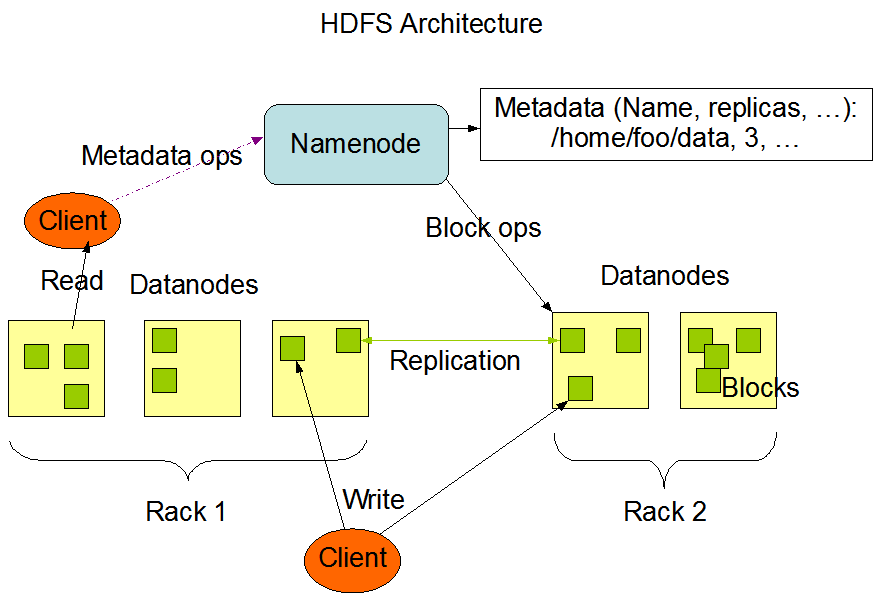
\includegraphics[width=1\textwidth]{hdfsarchitecture}}
\caption{Архитектура HDFS}
\label{fig:hdfsarchitecture}
\end{figure}

\begin{itemize}
\item \textbf{Namenode}

Этот компонент системы осуществляет всю работу с метаданными. Он должен быть запущен только на одном компьютере 
в кластере. Именно он управляет размещением информации и доступом ко всем данным, расположенным на ресурсах кластера. 
Сами данные проходят с остальных машин кластера к клиенту мимо него.

\item \textbf{Datanode}

На всех остальных компьютерах системы работает именно этот компонент. Он располагает сами блоки данных в локальной 
файловой системе для последующей передачи или обработки их по запросу клиента. Группы узлов данных принято называть 
Rack, они используются, например, в схемах репликации данных.

\item \textbf{Клиент}

Просто приложение или пользователь, работающий с файловой системой. В его роли может выступать практически что угодно.
\end{itemize}

Пространство имен HDFS имеет классическую иерархическую структуру: пользователи и приложения имеют возможность 
создавать директории и файлы. Файлы хранятся в виде блоков данных произвольной (но одинаковой, за исключением последнего; 
по-умолчанию 64 mb) длины, размещенных на Datanode'ах. Для обеспечения отказоустойчивости блоки хранятся в нескольких 
экземплярах на разных узлах, имеется возможность настройки количества копий и алгоритма их распределения по системе. 
Удаление файлов происходит не сразу, а через какое-то время после соответствующего запроса, так как после получения 
запроса файл перемещается в директорию /trash и хранится там определенный период времени на случай если пользователь 
или приложение передумают о своем решении. В этом случае информацию можно будет восстановить, в противном случае~--- физически удалить.

Для обнаружения возникновения каких-либо неисправностей, Datanode периодически отправляют Namenode'у сигналы о 
своей работоспособности. При прекращении получения таких сигналов от одного из узлов Namenode помечает его как <<мертвый>>, 
и прекращает какой-либо с ним взаимодействие до возвращения его работоспособности. Данные, хранившиеся на <<умершем>> узле 
реплицируются дополнительный раз из оставшихся <<в живых>> копий и система продолжает свое функционирование как ни в чем не бывало.

Все коммуникации между компонентами файловой системы проходят по специальным протоколам, основывающимся на стандартном TCP/IP. 
Клиенты работают с Namenode с помощью так называемого ClientProtocol, а передача данных происходит по DatanodeProtocol, 
оба они обернуты в Remote Procedure Call (RPC).

Система предоставляет несколько интерфейсов, среди которых командная оболочка DFSShell, набор ПО для администрирования DFSAdmin, 
а также простой, но эффективный веб-интерфейс. Помимо этого существуют несколько API для языков программирования: Java API, 
C pipeline, WebDAV и так далее.

\textbf{MapReduce}

Помимо файловой системы, Hadoop включает в себя framework для проведения масштабных вычислений, обрабатывающих 
огромные объемы данных. Каждое такое вычисление называется Job (задание) и состоит оно, как видно из названия, из двух этапов:

\begin{itemize}
\item \textbf{Map}

Целью этого этапа является представление произвольных данных (на практике чаще всего просто пары ключ-значение) в виде 
промежуточных пар ключ-значение. Результаты сортируются и групируются по ключу и передаются на следующий этап.

\item \textbf{Reduce}

Полученные после map значения используются для финального вычисления требуемых данных. Практические любые данные могут 
быть получены таким образом, все зависит от требований и функционала приложения.
\end{itemize}

Задания выполняются, подобно файловой системе, на всех машинах в кластере (чаще всего одних и тех же). Одна из них выполняет 
роль управления работой остальных — JobTracker, остальные же ее бесприкословно слушаются — TaskTracker. В задачи 
JobTracker'а входит составление расписания выполняемых работ, наблюдение за ходом выполнения, и перераспределение в случае 
возникновения сбоев.

В общем случае каждое приложение, работающее с этим framework'ом, предоставляет методы для осуществления этапов map и reduce, 
а также указывает расположения входных и выходных данных. После получения этих данных JobTracker распределяет задание между 
остальными машинами и предоставляет клиенту полную информацию о ходе работ.

Помимо основных вычислений могут выполняться вспомогательные процессы, такие как составление отчетов о ходе работы, кэширование, 
сортировка и так далее.

\textbf{HBase}

В рамках Hadoop доступна еще и система хранения данных, которую правда сложно назвать СУБД в традиционном смысле этого слова. 
Чаще проводят аналогии с проприетарной системой этого же плана от Google~--- BigTable.

HBase представляет собой распределенную систему хранения больших объемов данных. Подобно реляционным СУБД данные хранятся в 
виде таблиц, состоящих из строк и столбцов. И даже для доступа к ним предоставляется язык запросов HQL (как ни странно~--- 
Hadoop Query Language), отдаленно напоминающий более распространенный SQL. Помимо этого предоставляется итерирующмй интерфейс 
для сканирования наборов строк.

Одной из основных особенностей хранения данных в HBase является возможность наличия нескольких значений, 
соответствующих одной комбинации таблица-строка-столбец, для их различения используется информация о времени добавления записи. 
На концептуальном уровне таблицы обычно представляют как набор строк, но физически же они хранятся по столбцам, достаточно 
важный факт, который стоит учитывать при разработки схемы хранения данных. Пустые ячейки не отображаются каким-либо образом 
физически в хранимых данных, они просто отсутствуют. Существуют конечно и другие нюансы, но я постарался упомянуть лишь основные.

HQL очень прост по своей сути, если Вы уже знаете SQL, то для изучения его Вам понадобится лишь просмотреть по диагонали 
коротенький вывод команды help;, занимающий всего пару экранов в консоли. Все те же SELECT, INSERT, UPDATE, DROP и так далее, 
лишь со слегка измененным синтаксисом.

Помимо обычно командной оболочки HBase Shell, для работы с HBase также предоставлено несколько API для различных языков 
программирования: Java, Jython, REST и Thrift.

\textbf{HadoopDB}

В проекте HadoopDB специалисты из университетов Yale и Brown предпринимают попытку создать гибридную систему управления 
данными, сочетающую преимущества технологий и MapReduce, и параллельных СУБД. В их подходе MapReduce обеспечивает коммуникационную 
инфраструктуру, объединяющую произвольное число узлов, в которых выполняются экземпляры традиционной СУБД. Запросы формулируются 
на языке SQL, транслируются в среду MapReduce, и значительная часть работы передается в экземпляры СУБД. Наличие MapReduce 
обеспечивается масштабируемость и отказоустойчивость, а использование в узлах кластера СУБД позволяет добиться высокой 
производительности. 


\subsection{Установка и настройка}
Вся настройка ведется на Ubuntu Server операционной системе.

\subsubsection{Установка Hadoop}
Перед тем, как приступить собственно говоря к установке Hadoop, необходимо выполнить два элементарных действия, 
необходимых для правильного функционирования системы:
\begin{itemize}
\item открыть доступ одному из пользователей по ssh к этому же компьютеру без пароля, 
можно например создать отдельного пользователя для этого [hadoop]:
\begin{lstlisting}[label=lst:haddop1,caption=Создаем пользователя с правами]
$sudo groupadd hadoop
$sudo useradd -m -g hadoop -d /home/hadoop -s /bin/bash \
-c "Hadoop software owner" hadoop
\end{lstlisting}

Далее действия выполняем от его имени:
\begin{lstlisting}[label=lst:haddop2,caption=Логинимся под пользователем hadoop]
su hadoop
\end{lstlisting}

Генерим RSA-ключ для обеспечения аутентификации в условиях отсутствия возможности использовать пароль:
\begin{lstlisting}[label=lst:haddop3,caption=Генерим RSA-ключ]
hadoop@localhost ~ $ ssh-keygen -t rsa -P ""
Generating public/private rsa key pair.
Enter file in which to save the key (/home/hadoop/.ssh/id_rsa):
Your identification has been saved in /home/hadoop/.ssh/id_rsa.
Your public key has been saved in /home/hadoop/.ssh/id_rsa.pub.
The key fingerprint is:
7b:5c:cf:79:6b:93:d6:d6:8d:41:e3:a6:9d:04:f9:85 hadoop@localhost
\end{lstlisting}

И добавляем его в список авторизованных ключей:
\begin{lstlisting}[label=lst:haddop4,caption=Добавляем его в список авторизованных ключей]
cat $HOME/.ssh/id_rsa.pub >> $HOME/.ssh/authorized_keys
\end{lstlisting}

Этого должно быть более чем достаточно, проверить работоспособность соединения можно просто написав:
\begin{lstlisting}[label=lst:haddop5,caption=Пробуем зайти на ssh без пароля]
ssh localhost
\end{lstlisting}

Не забываем предварительно инициализировать sshd:
\begin{lstlisting}[label=lst:haddop6,caption=Запуск sshd]
/etc/init.d/sshd start
\end{lstlisting}

\item Помимо этого необходимо убедиться в наличии установленной JVM версии 1.5.0 или выше.
\begin{lstlisting}[label=lst:haddop7,caption=Устанавливаем JVM]
sudo aptitude install openjdk-6-jdk
\end{lstlisting}
\end{itemize}

Дальше скачиваем и устанавливаем Hadoop:
\begin{lstlisting}[label=lst:haddop8,caption=Устанавливаем Hadoop]
cd /opt
sudo wget http://www.gtlib.gatech.edu/pub/apache/hadoop
/core/hadoop-0.20.2/hadoop-0.20.2.tar.gz
sudo tar zxvf hadoop-0.20.2.tar.gz
sudo ln -s /opt/hadoop-0.20.2 /opt/hadoop
sudo chown -R hadoop:hadoop /opt/hadoop /opt/hadoop-0.20.2
sudo mkdir -p /opt/hadoop-data/tmp-base
sudo chown -R hadoop:hadoop /opt/hadoop-data/
\end{lstlisting}

Далее переходим в /opt/hadoop/conf/hadoop-env.sh и добавляем вначале:
\begin{lstlisting}[label=lst:haddop9,caption=Указываем переменные окружения]
export JAVA_HOME=/usr/lib/jvm/java-6-openjdk
export HADOOP_HOME=/opt/hadoop
export HADOOP_CONF=$HADOOP_HOME/conf
export HADOOP_PATH=$HADOOP_HOME/bin
export HIVE_HOME=/opt/hive
export HIVE_PATH=$HIVE_HOME/bin

export PATH=$HIVE_PATH:$HADOOP_PATH:$PATH
\end{lstlisting}

Далее добавим в /opt/hadoop/conf/hadoop-site.xml:
\begin{lstlisting}[language=XML,label=lst:haddop10,caption=Настройки hadoop]
<configuration>
<property>
  <name>hadoop.tmp.dir</name>
  <value>/opt/hadoop-data/tmp-base</value>
  <description>A base for other temporary directories</description>
</property>

<property>
  <name>fs.default.name</name>
  <value>localhost:54311</value>
  <description>
    The name of the default file system.
  </description>
</property>

<property>
  <name>hadoopdb.config.file</name>
  <value>HadoopDB.xml</value>
  <description>The name of the HadoopDB 
  cluster configuration file</description>
</property>
</configuration>
\end{lstlisting}

В /opt/hadoop/conf/mapred-site.xml:
\begin{lstlisting}[language=XML,label=lst:haddop11,caption=Настройки mapreduce]
<configuration>
<property>
  <name>mapred.job.tracker</name>
  <value>localhost:54310</value>
  <description>
    The host and port that the 
    MapReduce job tracker runs at.
  </description>
</property>
</configuration>
\end{lstlisting}

В /opt/hadoop/conf/hdfs-site.xml:
\begin{lstlisting}[language=XML,label=lst:haddop12,caption=Настройки hdfs]
<configuration>
<property>
  <name>dfs.replication</name>
  <value>1</value>
  <description>
    Default block replication.
  </description>
</property>
</configuration>
\end{lstlisting}

Теперь необходимо отформатировать Namenode:
\begin{lstlisting}[label=lst:haddop13,caption=Форматирование Namenode]
$ hadoop namenode -format
10/05/07 14:24:12 INFO namenode.NameNode: STARTUP_MSG: 
/************************************************************
STARTUP_MSG: Starting NameNode
STARTUP_MSG:   host = hadoop1/127.0.1.1
STARTUP_MSG:   args = [-format]
STARTUP_MSG:   version = 0.20.2
STARTUP_MSG:   build = https://svn.apache.org/repos
/asf/hadoop/common/branches/branch-0.20 -r
911707; compiled by 'chrisdo' on Fri Feb 19 08:07:34 UTC 2010
************************************************************/
10/05/07 14:24:12 INFO namenode.FSNamesystem: 
fsOwner=hadoop,hadoop
10/05/07 14:24:12 INFO namenode.FSNamesystem: 
supergroup=supergroup
10/05/07 14:24:12 INFO namenode.FSNamesystem: 
isPermissionEnabled=true
10/05/07 14:24:12 INFO common.Storage: 
Image file of size 96 saved in 0 seconds.
10/05/07 14:24:12 INFO common.Storage: 
Storage directory /opt/hadoop-data/tmp-base/dfs/name has been
successfully formatted.
10/05/07 14:24:12 INFO namenode.NameNode: 
SHUTDOWN_MSG: 
/************************************************************
SHUTDOWN_MSG: Shutting down NameNode at hadoop1/127.0.1.1
************************************************************/
\end{lstlisting}

Готово. Теперь мы можем запустить Hadoop:
\begin{lstlisting}[label=lst:haddop14,caption=Запуск Hadoop]
$ start-all.sh
starting namenode, logging to /opt/hadoop/bin/..
/logs/hadoop-hadoop-namenode-hadoop1.out
localhost: starting datanode, logging to 
/opt/hadoop/bin/../logs/hadoop-hadoop-datanode-hadoop1.out
localhost: starting secondarynamenode, logging to
/opt/hadoop/bin/../logs/hadoop-hadoop-secondarynamenode-hadoop1.out
starting jobtracker, logging to 
/opt/hadoop/bin/../logs/hadoop-hadoop-jobtracker-hadoop1.out
localhost: starting tasktracker, logging to
/opt/hadoop/bin/../logs/hadoop-hadoop-tasktracker-hadoop1.out
\end{lstlisting}

Остановка Hadoop производится скриптом stop-all.sh.

\subsubsection{Установка HadoopDB и Hive}
Теперь скачаем HaddopDB\footnote{http://sourceforge.net/projects/hadoopdb/files/} и распакуем hadoopdb.jar в \$HADOOP\_HOME/lib:
\begin{lstlisting}[label=lst:haddop15,caption=Установка HadoopDB]
$cp hadoopdb.jar $HADOOP_HOME/lib
\end{lstlisting}

Также нам потребуется PostgreSQL JDBC библиотека. Скачайте её\footnote{http://jdbc.postgresql.org/download.html} и 
распакуйте в директорию \$HADOOP\_HOME/lib.

Hive используется HadoopDB как SQL интерфейс. Подготовим директорию в HDFS для Hive:
\begin{lstlisting}[label=lst:haddop16,caption=Установка HadoopDB]
hadoop fs -mkdir /tmp
hadoop fs -mkdir /user/hive/warehouse
hadoop fs -chmod g+w /tmp
hadoop fs -chmod g+w /user/hive/warehouse
\end{lstlisting}

В архиве HadoopDB также есть архив SMS\_dist. Распакуем его:
\begin{lstlisting}[label=lst:haddop17,caption=Установка HadoopDB]
tar zxvf SMS_dist.tar.gz
sudo mv dist /opt/hive
sudo chown -R hadoop:hadoop hive
\end{lstlisting}

Поскольку мы успешно запустили Hadoop, то и проблем с запуском Hive не должно быть:
\begin{lstlisting}[label=lst:haddop18,caption=Установка HadoopDB]
$ hive
Hive history file=/tmp/hadoop/
hive_job_log_hadoop_201005081717_1990651345.txt
hive> 

hive> quit;
\end{lstlisting}

\subsubsection{Тестирование}
Теперь проведем тестирование. Для этого скачаем бенчмарк:
\begin{lstlisting}[label=lst:haddop19,caption=Тестирование]
svn co http://graffiti.cs.brown.edu/svn/benchmarks/
cd benchmarks/datagen/teragen
\end{lstlisting}

Изменим скрипт benchmarks/datagen/teragen/teragen.pl к виду:
\begin{lstlisting}[language=Java,label=lst:haddop20,caption=Тестирование]
use strict;
use warnings;

my $CUR_HOSTNAME = `hostname -s`;
chomp($CUR_HOSTNAME);

my $NUM_OF_RECORDS_1TB    = 10000000000;
my $NUM_OF_RECORDS_535MB  = 100;
my $BASE_OUTPUT_DIR   = "/data";
my $PATTERN_STRING    = "XYZ";
my $PATTERN_FREQUENCY = 108299;
my $TERAGEN_JAR       = "teragen.jar";
my $HADOOP_COMMAND    = $ENV{'HADOOP_HOME'}."/bin/hadoop";

my %files = ( "535MB" => 1,
);
system("$HADOOP_COMMAND fs -rmr $BASE_OUTPUT_DIR");
foreach my $target (keys %files) {
my $output_dir = $BASE_OUTPUT_DIR."/SortGrep$target";
my $num_of_maps = $files{$target};
my $num_of_records = ($target eq "535MB" ? 
$NUM_OF_RECORDS_535MB : $NUM_OF_RECORDS_1TB);
print "Generating $num_of_maps files in '$output_dir'\n";

##
## EXEC: hadoop jar teragen.jar 10000000000 
## /data/SortGrep/ XYZ 108299 100
##
my @args = ( $num_of_records,
	    $output_dir,
	    $PATTERN_STRING,
	    $PATTERN_FREQUENCY,
	    $num_of_maps );
my $cmd = "$HADOOP_COMMAND jar $TERAGEN_JAR ".join(" ", @args);
print "$cmd\n";
system($cmd) == 0 || die("ERROR: $!");
} # FOR
exit(0);
\end{lstlisting}

При запуске данного Perl скрипта сгенерится данные, которые будут сохранены на HDFS. 
Поскольку мы настроили систему как единственный кластер, то все данные будут загружены на один HDFS. 
При работе с большим количеством кластеров данные были бы распределены по кластерам.
Создадим базу данных, таблицу и загрузим данные, что мы сохранили на HDFS, в нее:
\begin{lstlisting}[label=lst:haddop21,caption=Тестирование]
$hadoop fs -get /data/SortGrep535MB/part-00000 my_file
$psql
psql> CREATE DATABASE grep0;
psql> USE grep0;
psql> CREATE TABLE grep (
    ->   key1 character varying(255),
    ->   field character varying(255)
    -> );
COPY grep FROM 'my_file' WITH DELIMITER '|';
\end{lstlisting}

Теперь настроим HadoopDB. В архиве HadoopDB можно найти пример файла Catalog.properties. Распакуйт его и настройте:
\begin{lstlisting}[label=lst:haddop22,caption=Тестирование]
#Properties for Catalog Generation
##################################
nodes_file=machines.txt
relations_unchunked=grep, EntireRankings
relations_chunked=Rankings, UserVisits
catalog_file=HadoopDB.xml
##
#DB Connection Parameters
##
port=5432
username=postgres
password=password
driver=com.postgresql.Driver
url_prefix=jdbc\:postgresql\://
##
#Chunking properties
##
chunks_per_node=0
unchunked_db_prefix=grep
chunked_db_prefix=cdb
##
#Replication Properties
##
dump_script_prefix=/root/dump_
replication_script_prefix=/root/load_replica_
dump_file_u_prefix=/mnt/dump_udb
dump_file_c_prefix=/mnt/dump_cdb
##
#Cluster Connection
##
ssh_key=id_rsa
\end{lstlisting}

Создайте файл machines.txt и добавте туда <<localhost>> строчку (без кавычек). Тепер создадим HadoopDB конфиг и скопируем его в HDFS:
\begin{lstlisting}[label=lst:haddop23,caption=Тестирование]
java -cp $HADOOP_HOME/lib/hadoopdb.jar \
> edu.yale.cs.hadoopdb.catalog.SimpleCatalogGenerator \
> Catalog.properties
hadoop dfs -put HadoopDB.xml HadoopDB.xml
\end{lstlisting}

Также возможно создать конфиг для создания репликации командой:
\begin{lstlisting}[label=lst:haddop23:1,caption=Репликация]
java -cp hadoopdb.jar edu.yale.cs.hadoopdb.catalog.SimpleRandomReplicationFactorTwo Catalog.properties
\end{lstlisting}

Инструмент генерирует новый файл HadoopDB.xml, в котором случайные порции данных реплицируются на все узлы.
После этого не забываем обновить конфиг на HDFS:
\begin{lstlisting}[label=lst:haddop23:2,caption=Обновляем конфиг]
hadoop dfs -rmr HadoopDB.xml
hadoop dfs -put HadoopDB.xml HadoopDB.xml
\end{lstlisting}
и поставить <<true>> для <<hadoopdb.config.replication>> в HADOOP\_HOME/conf/hadoop-site.xml.

Теперь мы готовы проверить работы HadoopDB. Теперь можем протестировать поиск по данным, загруженым ранее в БД и HDFS:
\begin{lstlisting}[label=lst:haddop24,caption=Тестирование]
java -cp $CLASSPATH:hadoopdb.jar \
> edu.yale.cs.hadoopdb.benchmark.GrepTaskDB \
> -pattern %wo% -output padraig -hadoop.config.file HadoopDB.xml
\end{lstlisting}

Приблизительный результат:
\begin{lstlisting}[label=lst:haddop25,caption=Тестирование]
$java -cp $CLASSPATH:hadoopdb.jar edu.yale.cs.hadoopdb.benchmark.GrepTaskDB \
> -pattern %wo% -output padraig -hadoop.config.file HadoopDB.xml
14.08.2010 19:08:48 edu.yale.cs.hadoopdb.exec.DBJobBase initConf
INFO: SELECT key1, field FROM grep WHERE field LIKE '%%wo%%';
14.08.2010 19:08:48 org.apache.hadoop.metrics.jvm.JvmMetrics init
INFO: Initializing JVM Metrics with processName=JobTracker, sessionId=
14.08.2010 19:08:48 org.apache.hadoop.mapred.JobClient configureCommandLineOptions
WARNING: Use GenericOptionsParser for parsing the arguments. 
Applications should implement Tool for the same.
14.08.2010 19:08:48 org.apache.hadoop.mapred.JobClient monitorAndPrintJob
INFO: Running job: job_local_0001
14.08.2010 19:08:48 edu.yale.cs.hadoopdb.connector.AbstractDBRecordReader getConnection
INFO: Data locality failed for leo-pgsql
14.08.2010 19:08:48 edu.yale.cs.hadoopdb.connector.AbstractDBRecordReader getConnection
INFO: Task from leo-pgsql is connecting to chunk 0 on host localhost with 
db url jdbc:postgresql://localhost:5434/grep0
14.08.2010 19:08:48 org.apache.hadoop.mapred.MapTask runOldMapper
INFO: numReduceTasks: 0
14.08.2010 19:08:48 edu.yale.cs.hadoopdb.connector.AbstractDBRecordReader close
INFO: DB times (ms): connection = 104, query execution = 20, row retrieval  = 79
14.08.2010 19:08:48 edu.yale.cs.hadoopdb.connector.AbstractDBRecordReader close
INFO: Rows retrieved = 3
14.08.2010 19:08:48 org.apache.hadoop.mapred.Task done
INFO: Task:attempt_local_0001_m_000000_0 is done. And is in the process of commiting
14.08.2010 19:08:48 org.apache.hadoop.mapred.LocalJobRunner$Job statusUpdate
INFO: 
14.08.2010 19:08:48 org.apache.hadoop.mapred.Task commit
INFO: Task attempt_local_0001_m_000000_0 is allowed to commit now
14.08.2010 19:08:48 org.apache.hadoop.mapred.FileOutputCommitter commitTask
INFO: Saved output of task 'attempt_local_0001_m_000000_0' to file:/home/leo/padraig
14.08.2010 19:08:48 org.apache.hadoop.mapred.LocalJobRunner$Job statusUpdate
INFO: 
14.08.2010 19:08:48 org.apache.hadoop.mapred.Task sendDone
INFO: Task 'attempt_local_0001_m_000000_0' done.
14.08.2010 19:08:49 org.apache.hadoop.mapred.JobClient monitorAndPrintJob
INFO:  map 100% reduce 0%
14.08.2010 19:08:49 org.apache.hadoop.mapred.JobClient monitorAndPrintJob
INFO: Job complete: job_local_0001
14.08.2010 19:08:49 org.apache.hadoop.mapred.Counters log
INFO: Counters: 6
14.08.2010 19:08:49 org.apache.hadoop.mapred.Counters log
INFO:   FileSystemCounters
14.08.2010 19:08:49 org.apache.hadoop.mapred.Counters log
INFO:     FILE_BYTES_READ=141370
14.08.2010 19:08:49 org.apache.hadoop.mapred.Counters log
INFO:     FILE_BYTES_WRITTEN=153336
14.08.2010 19:08:49 org.apache.hadoop.mapred.Counters log
INFO:   Map-Reduce Framework
14.08.2010 19:08:49 org.apache.hadoop.mapred.Counters log
INFO:     Map input records=3
14.08.2010 19:08:49 org.apache.hadoop.mapred.Counters log
INFO:     Spilled Records=0
14.08.2010 19:08:49 org.apache.hadoop.mapred.Counters log
INFO:     Map input bytes=3
14.08.2010 19:08:49 org.apache.hadoop.mapred.Counters log
INFO:     Map output records=3
14.08.2010 19:08:49 edu.yale.cs.hadoopdb.exec.DBJobBase run
INFO: 
JOB TIME : 1828 ms.

\end{lstlisting}

Результат сохранен в HDFS, в папке padraig:
\begin{lstlisting}[label=lst:haddop26,caption=Тестирование]
$ cd padraig
$ cat part-00000
some data
\end{lstlisting}

Проверим данные в PostgreSQL:
\begin{lstlisting}[label=lst:haddop27,caption=Тестирование]
psql> select * from grep where field like '%wo%';
+--------------------------------+-------------------+
| key1                           | field
|
+--------------------------------+-------------------+
some data

1 rows in set (0.00 sec)

psql>
\end{lstlisting}

Значения совадают. Все работает как требуется.

Проведем еще один тест. Добавим данные в PostgreSQL:
\begin{lstlisting}[label=lst:haddop27:1,caption=Тестирование]
psql> INSERT into grep(key1, field) VALUES('I am live!', 'Maybe');
psql> INSERT into grep(key1, field) VALUES('I am live!', 'Maybewqe');
psql> INSERT into grep(key1, field) VALUES('I am live!', 'Maybewqesad');
psql> INSERT into grep(key1, field) VALUES(':)', 'May cool string!');
\end{lstlisting}

Теперь проверим через HadoopDB:
\begin{lstlisting}[label=lst:haddop27:2,caption=Тестирование]
$ java -cp $CLASSPATH:hadoopdb.jar edu.yale.cs.hadoopdb.benchmark.GrepTaskDB -pattern %May% -output padraig -hadoopdb.config.file /opt/hadoop/conf/HadoopDB.xml
padraig
01.11.2010 23:14:45 edu.yale.cs.hadoopdb.exec.DBJobBase initConf
INFO: SELECT key1, field FROM grep WHERE field LIKE '%%May%%';
01.11.2010 23:14:46 org.apache.hadoop.metrics.jvm.JvmMetrics init
INFO: Initializing JVM Metrics with processName=JobTracker, sessionId=
01.11.2010 23:14:46 org.apache.hadoop.mapred.JobClient configureCommandLineOptions
WARNING: Use GenericOptionsParser for parsing the arguments. Applications should implement Tool for the same.
01.11.2010 23:14:46 org.apache.hadoop.mapred.JobClient monitorAndPrintJob
INFO: Running job: job_local_0001
01.11.2010 23:14:46 edu.yale.cs.hadoopdb.connector.AbstractDBRecordReader getConnection
INFO: Data locality failed for leo-pgsql
01.11.2010 23:14:46 edu.yale.cs.hadoopdb.connector.AbstractDBRecordReader getConnection
INFO: Task from leo-pgsql is connecting to chunk 0 on host localhost with db url jdbc:postgresql://localhost:5434/grep0
01.11.2010 23:14:47 org.apache.hadoop.mapred.MapTask runOldMapper
INFO: numReduceTasks: 0
01.11.2010 23:14:47 edu.yale.cs.hadoopdb.connector.AbstractDBRecordReader close
INFO: DB times (ms): connection = 181, query execution = 22, row retrieval  = 96
01.11.2010 23:14:47 edu.yale.cs.hadoopdb.connector.AbstractDBRecordReader close
INFO: Rows retrieved = 4
01.11.2010 23:14:47 org.apache.hadoop.mapred.Task done
INFO: Task:attempt_local_0001_m_000000_0 is done. And is in the process of commiting
01.11.2010 23:14:47 org.apache.hadoop.mapred.LocalJobRunner$Job statusUpdate
INFO: 
01.11.2010 23:14:47 org.apache.hadoop.mapred.Task commit
INFO: Task attempt_local_0001_m_000000_0 is allowed to commit now
01.11.2010 23:14:47 org.apache.hadoop.mapred.FileOutputCommitter commitTask
INFO: Saved output of task 'attempt_local_0001_m_000000_0' to file:/home/hadoop/padraig
01.11.2010 23:14:47 org.apache.hadoop.mapred.LocalJobRunner$Job statusUpdate
INFO: 
01.11.2010 23:14:47 org.apache.hadoop.mapred.Task sendDone
INFO: Task 'attempt_local_0001_m_000000_0' done.
01.11.2010 23:14:47 org.apache.hadoop.mapred.JobClient monitorAndPrintJob
INFO:  map 100% reduce 0%
01.11.2010 23:14:47 org.apache.hadoop.mapred.JobClient monitorAndPrintJob
INFO: Job complete: job_local_0001
01.11.2010 23:14:47 org.apache.hadoop.mapred.Counters log
INFO: Counters: 6
01.11.2010 23:14:47 org.apache.hadoop.mapred.Counters log
INFO:   FileSystemCounters
01.11.2010 23:14:47 org.apache.hadoop.mapred.Counters log
INFO:     FILE_BYTES_READ=141345
01.11.2010 23:14:47 org.apache.hadoop.mapred.Counters log
INFO:     FILE_BYTES_WRITTEN=153291
01.11.2010 23:14:47 org.apache.hadoop.mapred.Counters log
INFO:   Map-Reduce Framework
01.11.2010 23:14:47 org.apache.hadoop.mapred.Counters log
INFO:     Map input records=4
01.11.2010 23:14:47 org.apache.hadoop.mapred.Counters log
INFO:     Spilled Records=0
01.11.2010 23:14:47 org.apache.hadoop.mapred.Counters log
INFO:     Map input bytes=4
01.11.2010 23:14:47 org.apache.hadoop.mapred.Counters log
INFO:     Map output records=4
01.11.2010 23:14:47 edu.yale.cs.hadoopdb.exec.DBJobBase run
INFO: 
JOB TIME : 2332 ms.
\end{lstlisting}

Как паттерн поиска я задал <<May>>. В логах можно увидеть как производится поиск. На выходе получаем:
\begin{lstlisting}[label=lst:haddop27:3,caption=Тестирование]
$ cd padraig
$ cat part-00000
I am live!	Maybe
I am live!	Maybewqe
I am live!	Maybewqesad
:)	May cool string!
\end{lstlisting}

В упрощенной системе с одним кластером PostgreSQL не понятно ради чего такие сложности. 
Но если к HadoopDB подключить более одного кластера PostgreSQL, 
то данной методикой возможно работать с данными PostgreSQL, объединенных в shared-nothing кластер.

Более подробно по HadoopDB можно почитать по данной ссылке \\http://hadoopdb.sourceforge.net/guide/quick\_start\_guide.html.


\subsection{Заключение}
В данной статье не показывается, как работать с Hive, как более проще работать с HadoopDB. Эта книга не сможет учесть все, 
что требуется для работы c Hadoop. Назначение этой главы~--- дать основу для работы с Hadoop и HaddopDB.

HadoopDB не заменяет Hadoop. Эти системы сосуществуют, позволяя аналитику выбирать соответствующие средства в зависимости 
от имеющихся данных и задач.

HadoopDB может приблизиться в отношении производительности к параллельным системам 
баз данных, обеспечивая при этом отказоустойчивость и возможность использования в неоднородной среде при тех же правилах 
лицензирования, что и Hadoop. Хотя производительность HadoopDB, вообще говоря, ниже производительности параллельных систем 
баз данных, во многом это объясняется тем, что в PostgreSQL таблицы хранятся не по столбцам, и тем, что в PostgreSQL 
не использовалось сжатие данных. Кроме того, Hadoop и Hive~--- это сравнительно молодые проекты с открытыми кодами. 

В HadoopDB применяется некоторый гибрид подходов параллельных СУБД и Hadoop к анализу данных, позволяющий достичь производительности 
и эффективности параллельных систем баз данных, обеспечивая при этом масштабируемсть, отказоустойчивость и гибкость систем, 
основанных на MapReduce. Способность HadoopDB к прямому включению Hadoop и программного обеспечения СУБД с открытыми исходными 
текстами (без изменения кода) делает HadoopDB особенно пригодной для выполнения крупномасштабного анализа данных в будущих 
рабочих нагрузках.


\section{Заключение}
В данной главе расмотрено лиш базовые настройки кластеров БД. 
Про кластеры PostgreSQL потребуется написать отдельную книгу, чтобы растмотреть все шаги с установкой, настройкой и работой кластеров.
Надеюсь, что несмотря на это, информация будет полезна многим читателям.